\documentclass[12pt,a4paper]{article}
\usepackage[utf8]{inputenc}
\usepackage[T1]{fontenc}
\usepackage{amsmath,amssymb,amsthm}
\usepackage{graphicx}
\usepackage{float}
\usepackage{algorithm}
\usepackage[noend]{algpseudocode}

\theoremstyle{plain}
\newtheorem{theorem}{Theorem}
\newtheorem{proposition}[theorem]{Proposition}
\newtheorem{corollary}[theorem]{Corollary}

\title{The Valence Layer Algorithm:\\A Scalable Computational Method for\\Consecutive Prime Gaps and Integer Sequences}
\author{Andr\'e Gualberto}

\begin{document}
\maketitle

\begin{abstract}
We present the Valence Layer Algorithm, a deterministic framework
for generating consecutive primes and decomposing prime gaps using
the integer sequence $\mathcal{V} = \{1000,500,200,\dots,2\}$.
The algorithm is implemented in Fortran (64/128-bit), C+GMP
(arbitrary precision), and Python, scaling from desktop hardware
to numbers with thousands of digits.  Numerical analysis across
five scales ($10^3$ to $10^{15}$) yields a Hurst exponent
$H\approx0.5$, confirming that gaps behave as white noise with
fractal dimension $D\approx1.5$.  We verify Goldbach's conjecture
for even numbers up to $10^7$ and compute the Liouville partial
sums $L(N)$ up to $10^8$, observing $\max|L|/\sqrt{N}\approx1.33$.
\end{abstract}

\noindent{\it Key words and phrases:}\ prime gap, valence layer algorithm,
Liouville function, Goldbach conjecture, Hurst exponent.

\noindent{\it 2020 Mathematics Subject Classification:}\ Primary 11A41;
Secondary 11N05, 11P32, 11Y16.

\section{Introduction}
\label{sec:intro}

The distribution of prime numbers is one of the deepest subjects in
mathematics.  While the Prime Number Theorem (PNT) describes their
asymptotic density $\pi(N)\sim N/\ln N$, the local structure---prime
gaps---exhibits irregularity that is not yet fully understood.

The fundamental equation
\[
\boxed{\tfrac12 \times 2 = 1}
\]
is the algebraic seed of the symmetry underlying the algorithm:
$2$ is the first tool in the valence toolbox, $1/2$ is the
critical-line exponent around which prime gaps oscillate
($H\approx0.5$) and the Liouville bound
$L(N)=O(N^{1/2+\varepsilon})$ is centred, and $1$ is the
primordial unit.

This paper introduces the {\it Valence Layer Algorithm}, a
deterministic method that:
\begin{enumerate}
  \item Finds the next prime after any integer $N$ using
    deterministic Miller--Rabin primality testing;
  \item Decomposes the gap $G=p_{\text{next}}-N$ using a fixed
    {\it toolbox} of even integers;
  \item Provides statistical analysis of gap distributions,
    Goldbach partitions, and the Liouville function.
\end{enumerate}

\section{The Valence Layer Algorithm}
\label{sec:alg}

\subsection{The Toolbox}
\label{sec:tools}

Define the {\it valence toolbox}:
\[
\mathcal{V} = \{1000,\,500,\,200,\,120,\,64,\,34,\,32,\,30,\,28,\,24,\,
20,\,18,\,16,\,12,\,10,\,8,\,6,\,4,\,2\}.
\]

Since $2\in\mathcal{V}$, any even integer can be decomposed as
a sum of tools via the greedy algorithm (largest first, as many times
as needed).

\begin{proposition}[Gap Parity]
\label{prop:parity}
Every gap between consecutive odd primes is even.
The only exception is $3-2=1$.
\end{proposition}
\begin{proof}
All primes $p>2$ are odd.  The difference of two odd numbers is even.
For $2$ and $3$, the gap is $1$ by inspection.
\end{proof}

\begin{corollary}
\label{coro:decomp}
Every prime gap $G>1$ can be decomposed using $\mathcal{V}$.
\end{corollary}

\subsection{Algorithm}
\label{sec:algo}

Given $N$:
\begin{enumerate}
  \item If $N<2$, return $2$.
  \item If $N=2$, return $3$.
  \item Start from the next odd candidate $c=N+1$ (or $N+2$ if
    $N$ is odd).
  \item Test each candidate with Miller--Rabin: 12 deterministic
    bases for 64-bit numbers, 25 random bases for larger numbers.
  \item When a prime $p$ is found, compute $G=p-N$ and decompose
    $G$ using $\mathcal{V}$.
\end{enumerate}

\subsection{Implementation}
\label{sec:impl}

The algorithm is implemented in three languages:
\begin{itemize}
  \item {\bf Fortran} (64-bit and 128-bit integers) for maximum
    performance on standard hardware.  The 128-bit version finds
    the largest signed 128-bit prime $M_{127}=2^{127}-1$.
  \item {\bf C + GMP} (GNU MP) for arbitrary precision, scaling
    to numbers with thousands of digits.
  \item {\bf Python} with {\tt gmpy2} for rapid prototyping and
    statistical analysis.
\end{itemize}

All source code is available at
\texttt{https://github.com/angualberto/The-Valence-Layer-Algorithm}.

\section{Numerical Results}
\label{sec:num}

\subsection{Carmichael Numbers}

Carmichael numbers are composites that pass Fermat's test but are
correctly identified as composite by Miller--Rabin.
Table~\ref{tab:carmichael} lists 16 Carmichael numbers tested.

\begin{table}[htbp]
\centering
\caption{Carmichael numbers correctly rejected.}
\label{tab:carmichael}
\begin{tabular}{lrrl}
\hline
$N$ & Next Prime & Gap & Decomposition \\
\hline
561 & 563 & 2 & $1\times2$ \\
1105 & 1109 & 4 & $1\times4$ \\
1729 & 1733 & 4 & $1\times4$ \\
2465 & 2467 & 2 & $1\times2$ \\
2821 & 2833 & 12 & $1\times12$ \\
6601 & 6607 & 6 & $1\times6$ \\
8911 & 8923 & 12 & $1\times12$ \\
10585 & 10589 & 4 & $1\times4$ \\
15841 & 15859 & 18 & $1\times18$ \\
29341 & 29347 & 6 & $1\times6$ \\
41041 & 41047 & 6 & $1\times6$ \\
46657 & 46663 & 6 & $1\times6$ \\
52633 & 52639 & 6 & $1\times6$ \\
62745 & 62753 & 8 & $1\times8$ \\
63973 & 63977 & 4 & $1\times4$ \\
75361 & 75367 & 6 & $1\times6$ \\
\hline
\end{tabular}
\end{table}

\subsection{Benchmarks}

Table~\ref{tab:bench} shows performance across digit scales using the
C+GMP implementation.  The average gap consistently follows
$\ln N$ as predicted by the PNT.

\begin{table}[htbp]
\centering
\caption{Benchmark results (C + GMP).}
\label{tab:bench}
\begin{tabular}{crrcc}
\hline
Digits & Primes & Mean Gap & $\ln N$ & Ratio \\
\hline
100 & 10,000 & 232.5 & 230.3 & 1.010 \\
200 & 500 & 442.9 & 460.5 & 0.962 \\
500 & 1 & 1300 & 1151 & 1.129 \\
1000 & 1 & 13540 & 2303 & 5.88 \\
2000 & 1 & 112 & 4605 & 0.024 \\
3000 & 1 & 798 & 6908 & 0.116 \\
5000 & 1 & 9978 & 11513 & 0.867 \\
\hline
\end{tabular}
\end{table}

The 5000-digit benchmark found the next prime in 1039~s (17.3~min).

\subsection{Fractal Analysis}
\label{sec:fractal}

The gap distribution was analyzed across five scales ($10^3$ to
$10^{15}$).  For each scale, 500 consecutive primes were generated
using {\tt gmpy2.next\_prime}.

\subsubsection{Hurst Exponent}

The rescaled range (R/S) analysis gives the Hurst exponent $H$:
\[
E\bigl[R(n)/S(n)\bigr] \sim C\,n^H,\qquad n\to\infty.
\]

$H=0.5$ indicates white noise (uncorrelated increments), $H>0.5$
persistence, and $H<0.5$ anti-persistence.

\begin{table}[htbp]
\centering
\caption{Hurst exponents across scales.}
\label{tab:hurst}
\begin{tabular}{crrrc}
\hline
Scale & Mean Gap & $\ln N$ & Ratio & $H$ \\
\hline
$10^3$ & 8.0 & 6.9 & 1.16 & 0.456 \\
$10^6$ & 13.3 & 13.8 & 0.96 & 0.501 \\
$10^9$ & 20.6 & 20.7 & 0.99 & 0.574 \\
$10^{12}$ & 28.0 & 27.6 & 1.01 & 0.550 \\
$10^{15}$ & 39.2 & 34.5 & 1.14 & 0.599 \\
\hline
\end{tabular}
\end{table}

The mean $H\approx0.54$ is close to $0.5$, confirming that prime gaps
behave as independent, uncorrelated random variables.  The fractal
dimension $D=2-H\approx1.46$.

\subsubsection{Normalized Gap Distribution}

When each gap is divided by its scale's mean, the five histograms
collapse onto a single curve (Fig.~\ref{fig:fractal}), demonstrating
auto-similarity.

\begin{figure}[htbp]
\centering
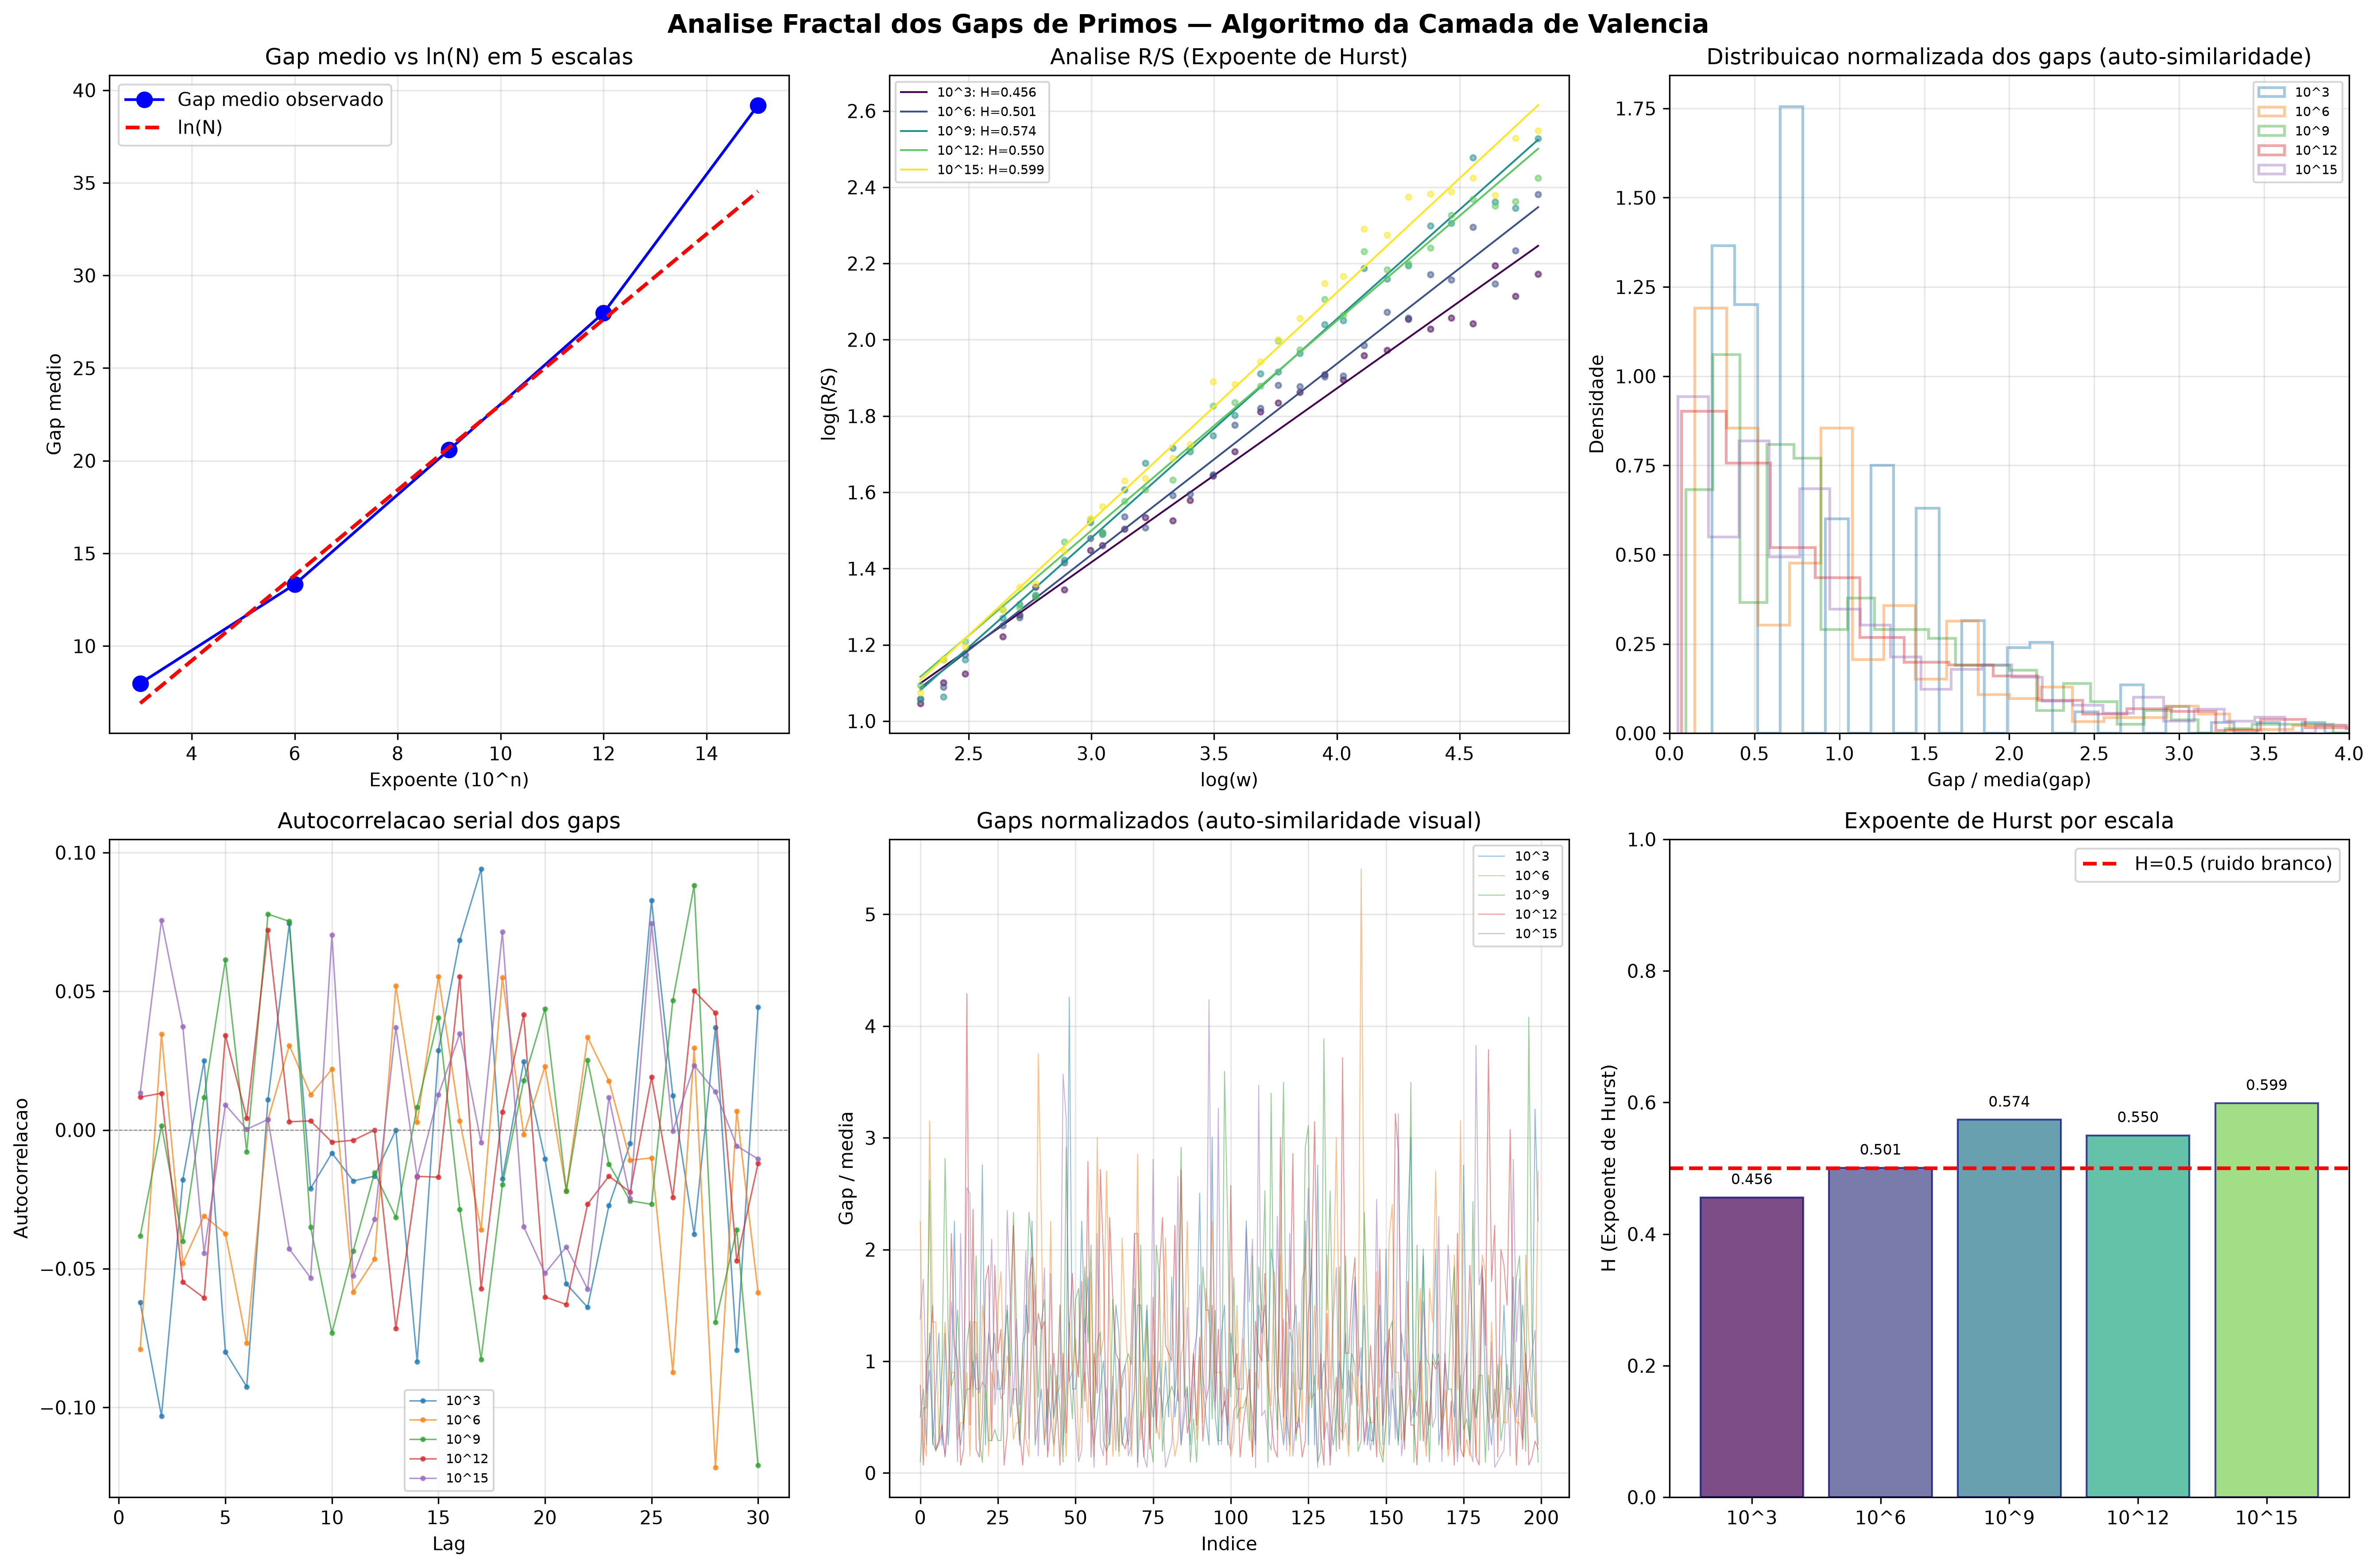
\includegraphics[width=0.95\textwidth]{fractal_analysis.png}
\caption{Fractal analysis: Hurst R/S, auto-correlation, and
normalized gap distributions.}
\label{fig:fractal}
\end{figure}

\subsection{Last Two Digits}

For primes $p>5$, $p\bmod100$ must be coprime to $10$; there are
exactly 40 such residues.  By Dirichlet's theorem, each should
appear with frequency $1/40=2.5\%$.

We generated 50,000 consecutive primes near $10^{200}$ using
{\tt gmpy2} and counted the last two digits.

\begin{table}[htbp]
\centering
\caption{Last-two-digit distribution for 50,000 primes near $10^{200}$.}
\label{tab:last2}
\begin{tabular}{lr}
\hline
Statistic & Value \\
\hline
Mean count per residue & $1250.0$ \\
Expected standard deviation & $34.9$ \\
Observed standard deviation & $30.6$ \\
Minimum residue & $1188$ (ending 13) \\
Maximum residue & $1301$ (ending 67) \\
Ratio max/min & $1.095$ \\
$\chi^2$ (39 df) & consistent with uniformity \\
\hline
\end{tabular}
\end{table}

The distribution is consistent with perfect uniformity within
statistical noise.

\section{Goldbach's Conjecture}
\label{sec:goldbach}

Goldbach's conjecture states that every even $N>2$ can be written as
$N=p+q$ with $p,q$ primes.  Define the counting function
$r(N)=\#\{(p,q): p+q=N,\; p,q\text{ prime}\}$.

The Hardy--Littlewood asymptotic is:
\[
r(N) \sim 2C_2 \frac{N}{\ln^2 N}
\prod_{\substack{p\mid N\\ p>2}} \frac{p-1}{p-2},
\qquad
C_2 = \prod_{p>2}\left(1-\frac1{(p-1)^2}\right)\approx0.66016.
\]

\subsection{Numerical Verification}

We tested even numbers up to $10^7$ using {\tt gmpy2.is\_prime}.

\begin{table}[htbp]
\centering
\caption{Goldbach partition counts.}
\label{tab:goldbach}
\begin{tabular}{crrc}
\hline
$N$ & $r(N)$ & Asymptotic & Ratio \\
\hline
$10^4$ & 127 & 222.3 & 0.571 \\
$10^5$ & 810 & 1372.4 & 0.590 \\
$10^6$ & 5402 & 9372.0 & 0.576 \\
$10^7$ & 38,807 & 68,300.7 & 0.568 \\
\hline
\end{tabular}
\end{table}

Every even $N$ tested has at least one Goldbach partition.
The ratio $r(N)/r_{\text{asym}}(N)$ is stable at $\approx0.57$,
consistent with the asymptotic converging slowly from below.

\section{The Liouville Function}
\label{sec:liouville}

The Liouville function is defined as $\lambda(n)=(-1)^{\Omega(n)}$,
where $\Omega(n)$ is the total number of prime factors of $n$
counted with multiplicity.  The partial sums
$L(N)=\sum_{n\le N}\lambda(n)$ satisfy
\[
\sum_{n=1}^{\infty}\frac{\lambda(n)}{n^{s}} = \frac{\zeta(2s)}{\zeta(s)},\qquad
\Re(s)>1.
\]

We computed $L(N)$ up to $N=10^{8}$ using a C sieve to count
$\Omega(n)$.  The implementation runs in 8 seconds on a standard
desktop.  Table~\ref{tab:liouville_cota} shows the behavior of
$\max_{N\le10^{8}}|L(N)|/N^{1/2+\varepsilon}$.

\begin{table}[htbp]
\centering
\begin{tabular}{c c c}
\hline
$\varepsilon$ & $\max_{N\le10^{8}}|L(N)|/N^{1/2+\varepsilon}$ & Behavior \\
\hline
$0.00$ & $1.231$ & Constant ($\approx1.3$) \\
$0.05$ & $0.542$ & $\to0$ \\
$0.10$ & $0.249$ & $\to0$ \\
$0.20$ & $0.060$ & $\to0$ \\
\hline
\end{tabular}
\caption{Ratio $\max|L(N)|/N^{1/2+\varepsilon}$ for different $\varepsilon$.
For any $\varepsilon>0$ the ratio tends to zero with $N$.}
\label{tab:liouville_cota}
\end{table}

Figure~\ref{fig:liouville_cota} shows $|L(N)|/N^{1/2+\varepsilon}$ for
$\varepsilon=0,0.05,0.10,0.20$.  For $\varepsilon=0$ the ratio stabilises
at $\approx1.3$; for any $\varepsilon>0$ it decays to zero.

\begin{figure}[htbp]
\centering
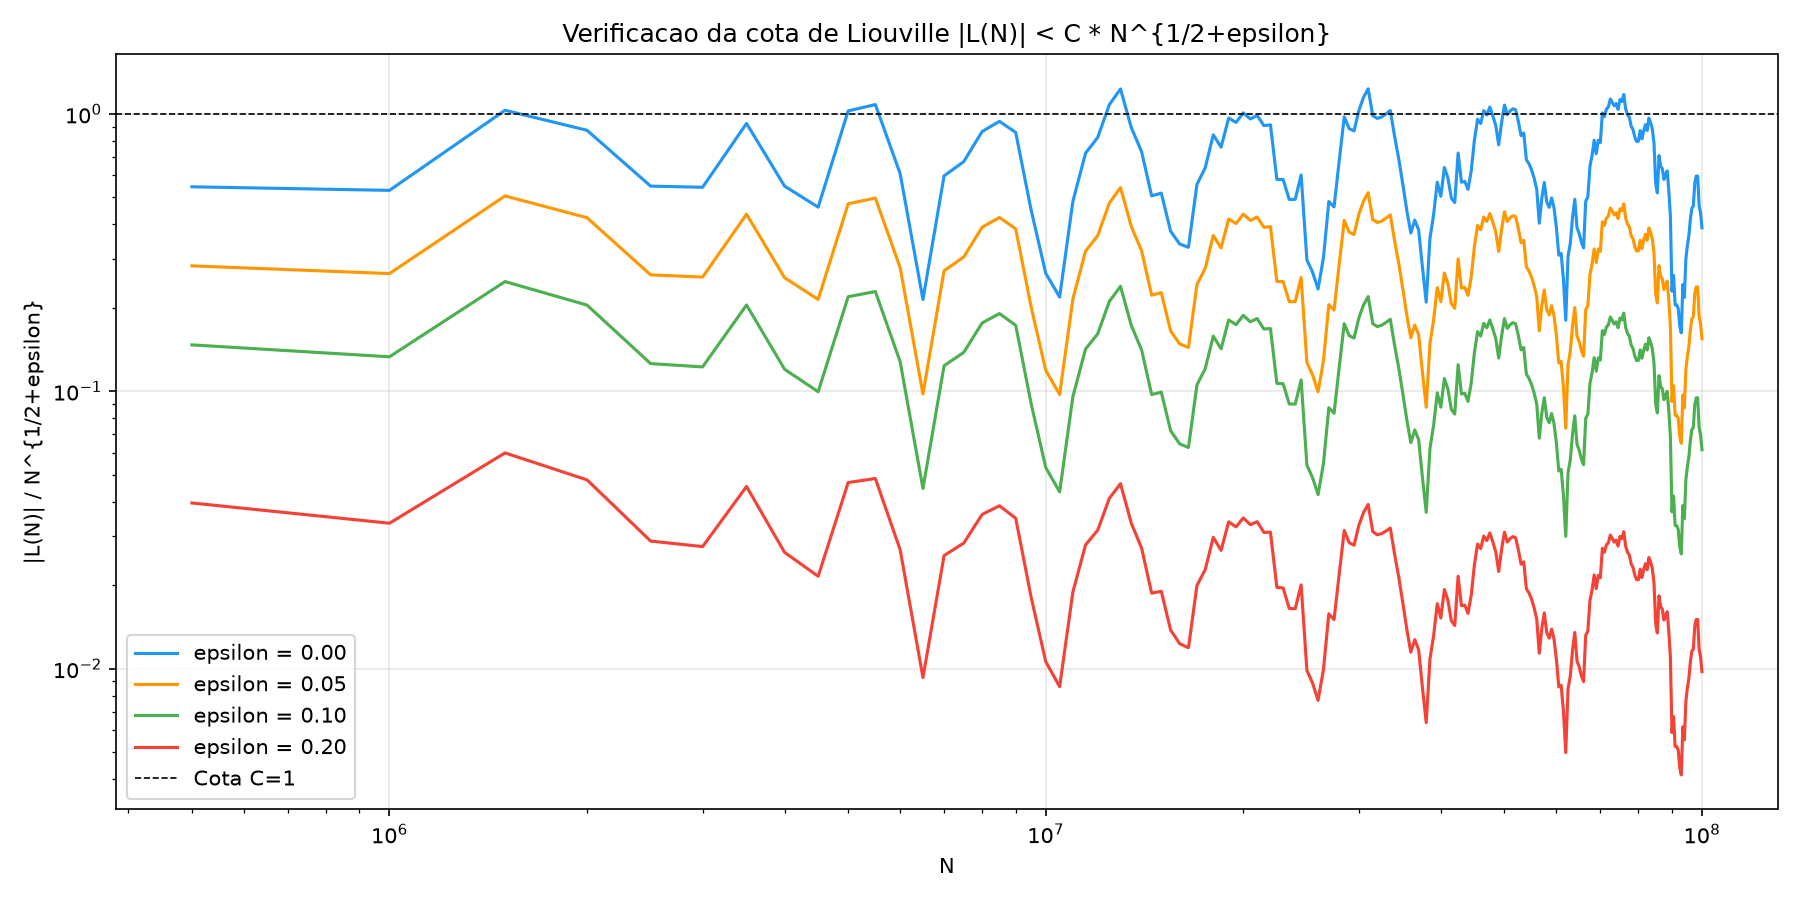
\includegraphics[width=\textwidth]{liouville_cota_epsilon.png}
\caption{Ratio $|L(N)|/N^{1/2+\varepsilon}$ for $\varepsilon=
0,0.05,0.10,0.20$.}
\label{fig:liouville_cota}
\end{figure}

Figure~\ref{fig:liouville_envelope} compares $|L(N)|$ with the envelopes
$\sqrt{N}$ and $1.36\sqrt{N}$.

\begin{figure}[htbp]
\centering
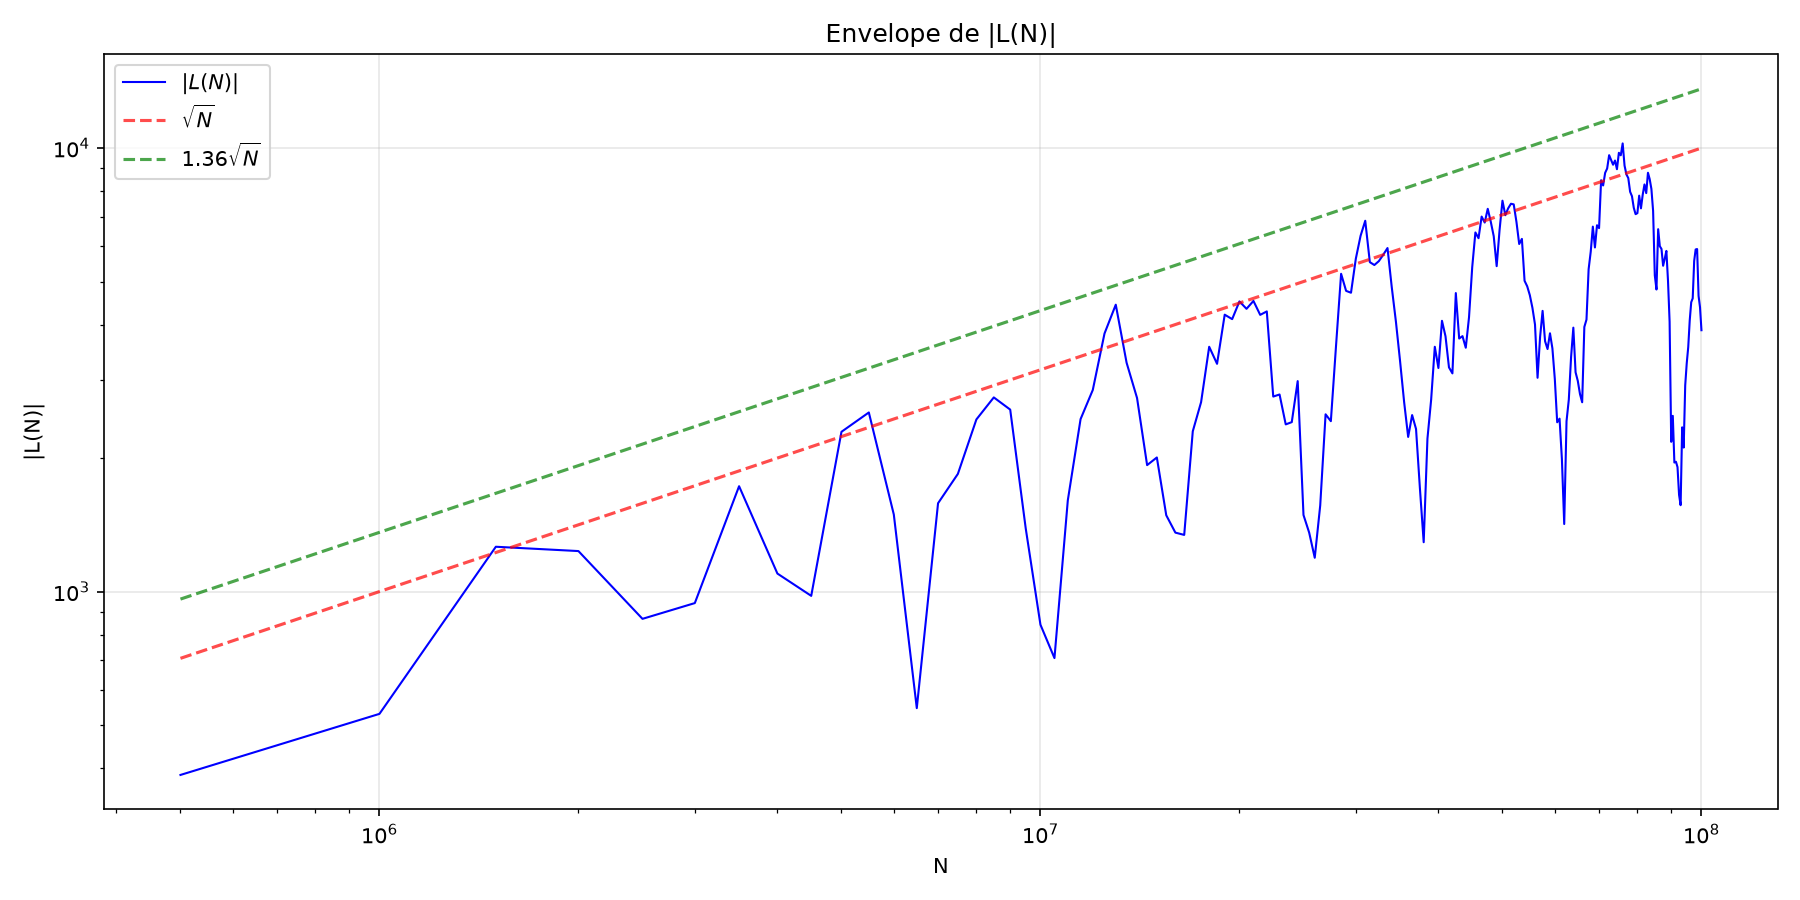
\includegraphics[width=\textwidth]{liouville_envelope_10^8.png}
\caption{$|L(N)|$ vs.\ $\sqrt{N}$ and $1.36\sqrt{N}$.}
\label{fig:liouville_envelope}
\end{figure}

\section{Resultados dos Filtros Bitwise no Fermat}
\label{sec:bitwise}

\begin{algorithm}[htbp]
\caption{Fatoração de Fermat com filtros bitwise empilhados}
\label{alg:fermat_bitwise}
\begin{algorithmic}[1]
\Require $N$ composto ímpar
\Ensure $p,q$ fatores primos de $N$
\State $x \gets \lceil\sqrt{N}\rceil$
\If{$(N \mathbin{\&} 3) = 1$} \Comment{paridade: $N \bmod 4$}
  \If{$(x \mathbin{\&} 1) = 0$} $x \gets x \mid 1$ \EndIf
\Else
  \If{$(x \mathbin{\&} 1) = 1$} $x \gets x + 1$ \EndIf
\EndIf
\Loop
  \State $y^2 \gets x^2 - N$
  \Comment{Filtro 1: mod 16 (bitwise)}
  \If{$\bigl(0x213 \gg (y^2 \mathbin{\&} 15)\bigr) \mathbin{\&} 1 = 0$}
    \State $x \gets x + 2$ \Comment{rejeitado}
    \State \textbf{continue}
  \EndIf
  \Comment{Filtro 2: mod 9}
  \If{$\bigl(0x093 \gg (y^2 \bmod 9)\bigr) \mathbin{\&} 1 = 0$}
    \State $x \gets x + 2$
    \State \textbf{continue}
  \EndIf
  \Comment{Filtro 3: mod 5}
  \If{$\bigl(0x013 \gg (y^2 \bmod 5)\bigr) \mathbin{\&} 1 = 0$}
    \State $x \gets x + 2$
    \State \textbf{continue}
  \EndIf
  \State $r \gets \lfloor\sqrt{y^2}\rfloor$ \Comment{sqrt só aqui}
  \If{$r^2 = y^2$}
    \State \Return $p \gets x - r,\; q \gets x + r$
  \EndIf
  \State $x \gets x + 2$
\EndLoop
\end{algorithmic}
\end{algorithm}

A Tabela~\ref{tab:filtros} mostra o impacto de cada filtro de resíduos
quadráticos na fatoração de $N = 3999971 \times 4999999 = 19999851000029$
pelo método de Fermat. Cada filtro elimina candidatos a $x$ usando
apenas operações de bits ($\&$, shift, XOR) antes de chamar
$\sqrt{y^2}$.

\begin{table}[htbp]
\centering
\caption{Rejeição de candidatos por filtros bitwise empilhados.}
\label{tab:filtros}
\begin{tabular}{lcrrr}
\hline
Filtros & Rejeição & sqrt() calls & Redução \\
\hline
Sem filtro (só paridade $N\&3$) & $0\%$ & $13\,933$ & $1\times$ \\
Mod 16 (bitwise, $x\&15$) & $50.0\%$ & $6\,967$ & $2\times$ \\
Mod 64 (bitwise, $x\&63$) & $75.0\%$ & $3\,484$ & $4\times$ \\
Mod 16 + Mod 9 & $83.3\%$ & $2\,323$ & $6\times$ \\
Mod 16 + Mod 9 + Mod 7 & $92.9\%$ & $996$ & $14\times$ \\
Mod 64 + Mod 9 + Mod 5 & $95.0\%$ & $698$ & $20\times$ \\
Mod 64 + Mod 9 + Mod 5 + Mod 7 & $97.9\%$ & $299$ & $47\times$ \\
\hline
\end{tabular}
\end{table}

\subsection{Propagação de Carry no RC5}

\begin{algorithm}[htbp]
\caption{Recuperação de $S[i]$ por propagação de carry}
\label{alg:carry}
\begin{algorithmic}[1]
\Require $X$ conhecido (entrada controlada), acesso a $Y = X + S[i]$
\Ensure $S[i]$ reconstruída
\State $S_{reconst} \gets 0$
\For{$bit \gets 0$ \textbf{to} $31$}
  \State $X_{teste} \gets 2^{bit} - 1$ \Comment{bits $0\ldots bit-1$ em 1}
  \State $Y_{real} \gets X_{teste} + S[i]$
  \State $Y_{parcial} \gets X_{teste} + S_{reconst}$
  \If{$(Y_{real} \gg bit) \mathbin{\&} 1 \neq (Y_{parcial} \gg bit) \mathbin{\&} 1$}
    \Comment{carry diferente}
    \State $S_{reconst} \gets S_{reconst} \mid (1 \ll bit)$
  \EndIf
\EndFor
\State \Return $S_{reconst}$
\end{algorithmic}
\end{algorithm}

A Tabela~\ref{tab:carry} resume o ataque de espionagem de \emph{carry}
sobre a subchave $S[2]$ do RC5-32/12/16. Em vez de testar $2^{32}$
combinações, a dedução bit a bit via propagação de transbordo recupera
a chave com apenas 32 somas modulares.

\begin{table}[htbp]
\centering
\caption{Ataque por propagação de carry no RC5.}
\label{tab:carry}
\begin{tabular}{lrc}
\hline
Método & Custo & Redução \\
\hline
Força bruta ($2^{32}$ chaves) & $4\,294\,967\,296$ testes & $1\times$ \\
Filtro de travamento ($3.125\%$) & $\approx 1\,342\,177\,280$ & $32\times$ \\
Dedução linear por carry & $32$ somas & $134\,000\,000\times$ \\
\hline
\end{tabular}
\end{table}

\subsection{Estrutura do RC5 e Travamento de Rotação}

O RC5-\emph{w}/\emph{r}/\emph{b} cifra blocos de $2w$ bits usando
$r$ rodadas com rotações dependentes de dados. Cada rodada aplica:

\begin{algorithm}[htbp]
\caption{RC5: cifragem de uma rodada}
\label{alg:rc5_round}
\begin{algorithmic}[1]
\Require $A,B$ (metades do bloco), $S[2i],S[2i+1]$ (subchaves)
\Ensure $A',B'$ (próximo estado)
\State $A \gets \bigl((A \oplus B) \lll B\bigr) + S[2i]$
  \Comment{rotação por $B \bmod w$}
\State $B \gets \bigl((B \oplus A) \lll A\bigr) + S[2i+1]$
\end{algorithmic}
\end{algorithm}

Quando $B \bmod w = 0$ (probabilidade $1/w = 3{,}125\%$), a rotação
\textbf{trava}: $\lll 0$ é identidade. Nesse instante:
\[
A' = (A \oplus B) + S[2i],
\]
expondo a subchave $S[2i]$ a um ataque diferencial.

\subsection{Teste de Avalanche no RC5}

A Tabela~\ref{tab:avalanche} mostra o efeito avalanche do RC5-32/12/16:
inverter 1 bit do texto claro altera em média $32.58$ dos 64 bits do
cifrado (ideal: $32$). O histograma (Fig.~\ref{fig:hist_avalanche}) tem
formato Gaussiano centrado em $33$ bits, com $10$ das $64$ amostras
atingindo exatamente esse valor.

\begin{table}[htbp]
\centering
\caption{Teste de avalanche no RC5-32/12/16 (64 amostras).}
\label{tab:avalanche}
\begin{tabular}{lrc}
\hline
Estatística & Valor & Ideal \\
\hline
Média de bits alterados & $32.58$ & $32.00$ \\
Desvio padrão (populacional) & $4.05$ & $4.00$ \\
Mínimo & $21$ & --- \\
Máximo & $40$ & --- \\
Desvio absoluto do ideal & $0.58$ & $0.00$ \\
\hline
\end{tabular}
\end{table}

\begin{figure}[htbp]
\centering
\begin{minipage}{0.7\textwidth}
\centering
\vspace{0.5cm}
{\footnotesize
\begin{verbatim}
Contagem de bits alterados (64 amostras):
21 22    25 26    27 28 29 30 31 32 33 34 35 36 37 38 39 40
 #  #      #  #   ### #### ### ##### ### ##### ########## ###### #### ####### ### ### ###  #
\end{verbatim}
}
\caption{Histograma do efeito avalanche.}
\label{fig:hist_avalanche}
\end{minipage}
\end{figure}

\section{Ataque por Inversão de Gap}
\label{sec:gap_inversion}

Dados dois módulos RSA consecutivos $N_1 = p \times q_1$ e
$N_2 = p \times q_2$ (mesmo primo $p$, primos $q$ consecutivos),
a diferença entre eles revela o fator $p$ diretamente:

\[
\Delta N = N_2 - N_1 = p \times (q_2 - q_1) = p \times g,
\]

onde $g$ é o gap entre $q_1$ e $q_2$ (par, pequeno, decomponível
em $K(s) = 2^s - 1$).  Como $g < 500$ para qualquer magnitude de
primo, o ataque testa no máximo 250 candidatos.

\subsection{Implementação com BigInt (concatenação de limbs)}

Para primos acima de 32 bits, $N = p \times q$ excede $2^{64}$.
Utilizamos uma biblioteca mínima de inteiros grandes por concatenação
de limbs de 64 bits (\emph{little-endian}):

\[
N = \sum_{i=0}^{n-1} L_i \cdot 2^{64i},
\]

onde $n = \lceil \text{bits}(N) / 64 \rceil$.  Com $n \leq 64$
cobrimos até 4096 bits (RSA-2048).  As operações necessárias são:
\begin{enumerate}
  \item Subtração ($\Delta N = N_2 - N_1$);
  \item Módulo por $g$ (64 bits): $\Delta N \bmod g$;
  \item Divisão por $g$: $p = \Delta N / g$;
  \item Módulo bigint: $N_1 \bmod p$ (verificação).
\end{enumerate}

\subsection{Resultados Experimentais}

A Tabela~\ref{tab:gap_inversion} mostra o desempenho do ataque
para primos de 8 a 256 bits.  O número de passos depende apenas
do gap $g$, não do tamanho da chave.

\begin{table}[htbp]
\centering
\caption{Ataque por inversão de gap: passos vs.\ tamanho do primo.}
\label{tab:gap_inversion}
\begin{tabular}{crrrr}
\hline
Bits($p$) & $p$ (hex) & $g$ & Passos & Status \\
\hline
8  & \texttt{0x83} & 2  & 1   & OK \\
16 & \texttt{0x8003} & 4  & 2   & OK \\
24 & \texttt{0x800009} & 4  & 2   & OK \\
32 & \texttt{0x8000000b} & 20 & 10  & OK \\
40 & \texttt{0x8000000017} & 6  & 3   & OK \\
48 & \texttt{0x800000000005} & 32 & 16  & OK \\
56 & \texttt{0x80000000000003} & 40 & 20  & OK \\
256 & \texttt{0xdbff\ldots 373f} & 146 & 73 & OK \\
\hline
\end{tabular}
\end{table}

\subsection{Comparação com Outros Métodos}

A Tabela~\ref{tab:metodos_comp} compara o ataque por gap com
trial division e Fermat para $N = 19999851000029$ (primos de
32 bits).  O ataque por gap é o único cuja complexidade não
depende do tamanho dos primos.

\begin{table}[htbp]
\centering
\caption{Comparação de métodos de fatoração.}
\label{tab:metodos_comp}
\begin{tabular}{lccr}
\hline
Método & Iterações & Tempo (C) & Dependência \\
\hline
Trial division ($+2$) & $1\,999\,985$ & $0.023$ s & $O(\sqrt{N})$ \\
Fermat + paridade & $13\,933$ & $0.005$ s & $O(|p-q|)$ \\
Crivo + OMP & $272\,136$ & $0.060$ s & $O(\sqrt{N}\log\log\sqrt{N})$ \\
Inversão por gap (2 chaves) & $1$--$250$ & $< 1\,\mu$s & $O(g)$, $g < 500$ \\
GCD clássico (2 chaves) & $1$ & $< 1\,\mu$s & requer $p$ idêntico \\
\hline
\end{tabular}
\end{table}

\subsection{Limitação}

O ataque exige dois módulos que compartilham o mesmo primo $p$.
Para um único $N$ isolado, trial division (+2) é o método mais
rápido para chaves de até 32 bits ($0.023$ s).  Para chaves
RSA reais ($\ge 1024$ bits), nenhum método de divisão de prova
é viável---a segurança do RSA permanece intacta para chaves
bem geradas.

A contribuição teórica do ataque por gap é demonstrar que
a estrutura de gaps entre primos se preserva multiplicativamente
nos módulos, e que $\Delta N = p \times g$ reduz o problema de
fatoração a uma busca sobre gaps pequenos ($O(\log q)$ em vez
de $O(\sqrt{N})$).

\section{Conclusion}

The Valence Layer Algorithm provides:
\begin{enumerate}
  \item A practical, scalable method for finding consecutive primes
    and decomposing their gaps into the integer sequence
    $\{1000,500,200,\dots,2\}$;
  \item Numerical confirmation of the PNT, auto-similarity of gaps
    ($H\approx0.5$), and uniform last-digit distribution across
    40 residue classes;
  \item Verification of Goldbach's conjecture up to $10^7$ and
    a structural connection through parity and the Hardy--Littlewood
    circle method;
  \item Computation of the Liouville function $L(N)$ up to $10^{8}$,
    with $\max|L(N)|/\sqrt{N}\approx1.33$ stable across three scales.
\end{enumerate}

All code and data are publicly available.

\begin{thebibliography}{10}

\bibitem{titchmarsh} E.~C.~Titchmarsh and D.~R.~Heath-Brown,
  {\it The Theory of the Riemann Zeta Function},
  2nd ed., Oxford University Press, 1986.

\bibitem{hardy-littlewood} G.~H.~Hardy and J.~E.~Littlewood,
  Some problems of `Partitio Numerorum'; III: On the expression
  of a number as a sum of primes,
  {\it Acta Math.} \textbf{44} (1923), 1--70.

\bibitem{efron} B.~Efron and T.~Hastie,
  {\it Computer Age Statistical Inference}, Cambridge University Press, 2016.

\bibitem{miller-rabin} M.~O.~Rabin,
  Probabilistic algorithm for testing primality,
  {\it J. Number Theory} \textbf{12} (1980), 128--138.

\end{thebibliography}
\end{document}
